% Chapter 4: SARIMA Models
% Harvard-quality academic presentation
% Bachelor program, Bucharest University of Economic Studies

\documentclass[9pt, aspectratio=169, t]{beamer}

% Ensure content fits on slides
\setbeamersize{text margin left=8mm, text margin right=8mm}

%=============================================================================
% THEME AND STYLE CONFIGURATION
%=============================================================================
\usetheme{default}
% Using default theme for clean header/footer control

% Color Palette (matching Redispatch PDF)
\definecolor{MainBlue}{RGB}{26, 58, 110}
\definecolor{AccentBlue}{RGB}{26, 58, 110}
\definecolor{IDAred}{RGB}{205, 0, 0}
\definecolor{DarkGray}{RGB}{51, 51, 51}
\definecolor{MediumGray}{RGB}{128, 128, 128}
\definecolor{LightGray}{RGB}{248, 248, 248}
\definecolor{VeryLightGray}{RGB}{235, 235, 235}
\definecolor{KeynoteGray}{RGB}{218, 218, 218}
\definecolor{SectionGray}{RGB}{120, 120, 120}
\definecolor{FooterGray}{RGB}{100, 100, 100}
\definecolor{Crimson}{RGB}{220, 53, 69}
\definecolor{Forest}{RGB}{46, 125, 50}
\definecolor{Amber}{RGB}{181, 133, 63}
\definecolor{Orange}{RGB}{230, 126, 34}
\definecolor{Purple}{RGB}{142, 68, 173}

% Gradient background (exact Keynote 315° gradient: white to RGB 218,218,218)
\setbeamertemplate{background}{%
    \begin{tikzpicture}[remember picture, overlay]
        \shade[shading=axis, shading angle=315,
        top color=white, bottom color=KeynoteGray]
        (current page.south west) rectangle (current page.north east);
    \end{tikzpicture}%
}
% Fallback solid color for compatibility
\setbeamercolor{background canvas}{bg=}

\setbeamercolor{palette primary}{bg=MainBlue, fg=white}
\setbeamercolor{palette secondary}{bg=MainBlue!85, fg=white}
\setbeamercolor{palette tertiary}{bg=MainBlue!70, fg=white}
\setbeamercolor{structure}{fg=MainBlue}
\setbeamercolor{title}{fg=IDAred}
\setbeamercolor{frametitle}{fg=IDAred, bg=}
\setbeamercolor{block title}{bg=MainBlue, fg=white}
\setbeamercolor{block body}{bg=VeryLightGray, fg=DarkGray}
\setbeamercolor{block title alerted}{bg=Crimson, fg=white}
\setbeamercolor{block body alerted}{bg=Crimson!8, fg=DarkGray}
\setbeamercolor{block title example}{bg=Forest, fg=white}
\setbeamercolor{block body example}{bg=Forest!8, fg=DarkGray}
\setbeamercolor{item}{fg=MainBlue}

% Footer colors (override Madrid theme blue)
\setbeamercolor{author in head/foot}{fg=FooterGray, bg=}
\setbeamercolor{title in head/foot}{fg=FooterGray, bg=}
\setbeamercolor{date in head/foot}{fg=FooterGray, bg=}
\setbeamercolor{section in head/foot}{fg=FooterGray, bg=}
\setbeamercolor{subsection in head/foot}{fg=FooterGray, bg=}

% Bullet styles (apply everywhere including blocks)
\setbeamertemplate{itemize item}{\color{MainBlue}$\boxdot$}
\setbeamertemplate{itemize subitem}{\color{MainBlue}$\blacktriangleright$}
\setbeamertemplate{itemize subsubitem}{\color{MainBlue}\tiny$\bullet$}
\setbeamertemplate{itemize/enumerate body begin}{\normalsize}
\setbeamertemplate{itemize/enumerate subbody begin}{\normalsize}

% Item spacing
\setlength{\leftmargini}{1.5em}
\setlength{\leftmarginii}{1.5em}

\setbeamertemplate{navigation symbols}{}

% TOC with bullets
\setbeamertemplate{section in toc}{\color{MainBlue}$\boxdot$\hspace{0.5em}\inserttocsection}

%=============================================================================
% CUSTOM HEADLINE
%=============================================================================
\setbeamertemplate{headline}{%
    \vskip10pt%
    \hbox to \paperwidth{%
        \hskip0.5cm%
        {\small\color{FooterGray}\renewcommand{\hyperlink}[2]{##2}\insertsectionhead}%
        \hfill%
        \textcolor{FooterGray}{\small\insertframenumber}%
        \hskip0.5cm%
    }%
    \vskip4pt%
    {\color{FooterGray}\hrule height 0.4pt}%
}

%=============================================================================
% CUSTOM FOOTER
%=============================================================================
\usepackage{fontawesome5}

\setbeamertemplate{footline}{%
    {\color{FooterGray}\hrule height 0.4pt}%
    \vskip4pt%
    \hbox to \paperwidth{%
        \hskip0.5cm%
        \textcolor{FooterGray}{\small Time Series Analysis and Forecasting}%
        \hfill%
        \raisebox{-0.1em}{%
            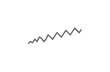
\begin{tikzpicture}[x=0.08em, y=0.08em, line width=0.4pt]
                \draw[FooterGray] (0,3) -- (1,4) -- (2,3.5) -- (3,5) -- (4,4) -- (5,6) -- (6,5.5) -- (7,4) -- (8,5) -- (9,7) -- (10,6) -- (11,5) -- (12,6.5) -- (13,8) -- (14,7) -- (15,6) -- (16,7.5) -- (17,9) -- (18,8) -- (19,7) -- (20,8.5) -- (21,10) -- (22,9) -- (23,8) -- (24,9.5);
            \end{tikzpicture}%
        }%
        \hskip0.5cm%
    }%
    \vskip6pt%
}

%=============================================================================
% PACKAGES
%=============================================================================
\usepackage[utf8]{inputenc}
\usepackage[T1]{fontenc}
\usepackage{amsmath, amssymb, amsthm}
\usepackage{mathtools}
\usepackage{bm}
\usepackage{tikz}
\usetikzlibrary{arrows.meta, positioning, shapes, calc, decorations.pathreplacing, shadings}
\usepackage{booktabs}
\usepackage{multirow}
\usepackage{array}
\usepackage{graphicx}
\usepackage{hyperref}
\usepackage{colortbl}
\hypersetup{colorlinks=true, linkcolor=MainBlue, urlcolor=MainBlue}
\graphicspath{{../logos/}{../charts/}}

%=============================================================================
% QUANTLET COMMAND
%=============================================================================
\newcommand{\quantlet}[2]{%
    \begin{tikzpicture}[remember picture, overlay]
        \node[anchor=south east, inner sep=0pt] at ([xshift=-0.5cm, yshift=0.75cm]current page.south east) {%
            \href{#2}{%
                \raisebox{-0.1em}{\includegraphics[height=0.8em]{ql_logo.png}}%
                \textcolor{MainBlue}{\scriptsize\ #1}%
            }%
        };
    \end{tikzpicture}%
}

%=============================================================================
% CUSTOM TITLE PAGE
%=============================================================================
\defbeamertemplate*{title page}{hybrid}[1][]
{
    \vspace{0.2cm}
    % Logos row - top header (with clickable links)
    \begin{center}
        \href{https://www.ase.ro}{\includegraphics[height=0.9cm]{ase_logo.png}}\hspace{0.15cm}%
        \href{https://theida.net}{\includegraphics[height=0.9cm]{ida_logo.png}}\hspace{0.15cm}%
        \href{https://blockchain-research-center.com}{\includegraphics[height=0.9cm]{brc_logo.png}}\hspace{0.15cm}%
        \href{https://www.ai4efin.ase.ro}{\includegraphics[height=0.9cm]{ai4efin_logo.png}}\hspace{0.15cm}%
        \href{https://ipe.ro/new}{\includegraphics[height=0.9cm]{acad_logo.png}}\hspace{0.15cm}%
        \href{https://www.digital-finance-msca.com}{\includegraphics[height=0.9cm]{msca_logo.png}}%
    \end{center}

    \vspace{0.6cm}

    % Main title with Q logos on sides (with clickable links)
    \begin{center}
        \begin{minipage}{0.1\textwidth}
            \centering
            \href{https://quantlet.com}{\includegraphics[height=1.1cm]{ql_logo.png}}
        \end{minipage}%
        \begin{minipage}{0.76\textwidth}
            \centering
            {\LARGE\bfseries\usebeamercolor[fg]{title}\inserttitle}

            \vspace{0.3cm}

            {\usebeamerfont{subtitle}\usebeamercolor[fg]{title}\insertsubtitle}
        \end{minipage}%
        \begin{minipage}{0.1\textwidth}
            \centering
            \href{https://quantinar.com}{\includegraphics[height=1.1cm]{qr_logo.png}}
        \end{minipage}
    \end{center}

    \vspace{0.6cm}

    % Authors (left aligned)
    \hspace{0.5cm}{\usebeamerfont{author}\insertauthor}

    \vspace{0.3cm}

    % Institute/Affiliations (left aligned)
    \hspace{0.5cm}\begin{minipage}[t]{0.9\textwidth}
        \raggedright\small\insertinstitute
    \end{minipage}
}

%=============================================================================
% THEOREM ENVIRONMENTS
%=============================================================================
\theoremstyle{definition}
\setbeamertemplate{theorems}[numbered]
\newtheorem{defn}{Definition}
\newtheorem{thm}{Theorem}
\newtheorem{prop}{Proposition}
\newtheorem{rmk}{Remark}

%=============================================================================
% CUSTOM COMMANDS
%=============================================================================
\newcommand{\E}{\mathbb{E}}
\newcommand{\Var}{\text{Var}}
\newcommand{\Cov}{\text{Cov}}
\newcommand{\Corr}{\text{Corr}}
\newcommand{\R}{\mathbb{R}}
\newcommand{\N}{\mathbb{N}}
\newcommand{\Z}{\mathbb{Z}}
\newcommand{\B}{\mathbf{B}}
\newcommand{\imark}{\textcolor{MainBlue}{\textbullet}}
\newcommand{\RMSE}{\text{RMSE}}
\newcommand{\MAE}{\text{MAE}}
\newcommand{\MAPE}{\text{MAPE}}

%=============================================================================
% TITLE INFORMATION
%=============================================================================
\title[Time Series Analysis]{Time Series Analysis and Forecasting}
\subtitle{Chapter 4: SARIMA Models}
\author[D.T. Pele]{Daniel Traian PELE}
\institute{Bucharest University of Economic Studies\\
IDA Institute Digital Assets\\
Blockchain Research Center\\
AI4EFin Artificial Intelligence for Energy Finance\\
Romanian Academy, Institute for Economic Forecasting\\
MSCA Digital Finance}
\date{}

\begin{document}

% Title page (no header/footer)
{
\setbeamertemplate{headline}{}
\setbeamertemplate{footline}{}
\begin{frame}
    \titlepage
\end{frame}
}

%=============================================================================
% TABLE OF CONTENTS
%=============================================================================
\begin{frame}{Outline}
    \tableofcontents
\end{frame}

%=============================================================================
% MOTIVATION
%=============================================================================
\section{Motivation}

\begin{frame}{Motivating Example: Seasonality Is Everywhere}
    \vspace{-0.3cm}
    \begin{center}
        \includegraphics[width=0.88\textwidth, height=0.62\textheight, keepaspectratio]{charts/ch4_motivation_seasonal.pdf}
    \end{center}
    \vspace{-0.2cm}
    {\footnotesize
    \begin{itemize}
        \item Retail sales exhibit clear \textbf{annual patterns}: December peaks, January troughs
        \item Standard ARIMA models cannot capture these \textbf{repeating seasonal cycles}
        \item Ignoring seasonality leads to systematic forecast errors
    \end{itemize}
    }
    \quantlet{TSA\_ch4\_motivation\_seasonal}{https://github.com/QuantLet/TSA/tree/main/TSA_ch4/TSA_ch4_motivation_seasonal}
\end{frame}

\begin{frame}{Understanding Seasonal Components}
    \vspace{-0.3cm}
    \begin{center}
        \includegraphics[width=0.88\textwidth, height=0.62\textheight, keepaspectratio]{charts/ch4_motivation_decomposition.pdf}
    \end{center}
    \vspace{-0.2cm}
    {\footnotesize
    \begin{itemize}
        \item Seasonal time series = \textbf{Trend} + \textbf{Seasonal Pattern} + \textbf{Residuals}
        \item Decomposition helps visualize each component separately
        \item SARIMA models capture both trend dynamics and seasonal behavior
    \end{itemize}
    }
    \quantlet{TSA\_ch4\_motivation\_decomposition}{https://github.com/QuantLet/TSA/tree/main/TSA_ch4/TSA_ch4_motivation_decomposition}
\end{frame}

\begin{frame}{Real-World Application: Monthly Patterns}
    \vspace{-0.3cm}
    \begin{center}
        \includegraphics[width=0.88\textwidth, height=0.62\textheight, keepaspectratio]{charts/ch4_motivation_monthly.pdf}
    \end{center}
    \vspace{-0.2cm}
    {\footnotesize
    \begin{itemize}
        \item Energy demand shows strong \textbf{monthly seasonality}
            \begin{itemize}
                \item Heating cycles in winter, cooling cycles in summer
            \end{itemize}
        \item Pattern repeats predictably each year with slight weather variations
        \item Utility companies use SARIMA forecasts for capacity planning
    \end{itemize}
    }
    \quantlet{TSA\_ch4\_motivation\_monthly}{https://github.com/QuantLet/TSA/tree/main/TSA_ch4/TSA_ch4_motivation_monthly}
\end{frame}

\begin{frame}{Why Do We Need SARIMA?}
    \vspace{-0.3cm}
    \begin{center}
        \includegraphics[width=0.88\textwidth, height=0.62\textheight, keepaspectratio]{charts/ch4_motivation_why_sarima.pdf}
    \end{center}
    \vspace{-0.2cm}
    {\footnotesize
    \begin{itemize}
        \item \textbf{Left}: Seasonal ACF patterns --- spikes at lags 12, 24, 36 reveal annual cycle
        \item \textbf{Right}: ARIMA residuals still show seasonal autocorrelation (incomplete model)
        \item \textbf{SARIMA solution}: Adds seasonal AR/MA terms to capture periodic patterns
    \end{itemize}
    }
    \quantlet{TSA\_ch4\_motivation\_why\_sarima}{https://github.com/QuantLet/TSA/tree/main/TSA_ch4/TSA_ch4_motivation_why_sarima}
\end{frame}

\begin{frame}{What We'll Learn Today}
    {\small
    \hfill\begin{minipage}{0.9\textwidth}
        \begin{columns}[T]
            \begin{column}{0.48\textwidth}
                \begin{block}{Concepts}
                    \begin{itemize}\setlength{\itemsep}{1pt}
                        \item Identifying seasonal patterns
                        \item Seasonal differencing operator
                        \item SARIMA$(p,d,q)(P,D,Q)_s$ notation
                        \item The famous ``Airline Model''
                        \item Model selection for seasonal data
                    \end{itemize}
                \end{block}
            \end{column}
            \begin{column}{0.48\textwidth}
                \begin{block}{Skills}
                    \begin{itemize}\setlength{\itemsep}{1pt}
                        \item Diagnose seasonality from ACF/PACF
                        \item Determine seasonal period $s$
                        \item Choose $(P, D, Q)$ seasonal orders
                        \item Implement SARIMA in Python/R
                        \item Forecast seasonal time series
                    \end{itemize}
                \end{block}
            \end{column}
        \end{columns}
    \end{minipage}
    }

    \vspace{0.3cm}

    \begin{alertblock}{Key Insight}
        SARIMA = ARIMA applied at \textbf{two frequencies}: the regular (short-term) and seasonal (long-term) levels
    \end{alertblock}
\end{frame}

%=============================================================================
% SECTION 1: SEASONALITY IN TIME SERIES
%=============================================================================
\section{Seasonality in Time Series}

\begin{frame}{What is Seasonality?}
    \begin{defn}[Seasonality]
        A time series exhibits \textbf{seasonality} when it shows regular, periodic fluctuations that repeat over a fixed period $s$ (the seasonal period).
    \end{defn}

    \vspace{0.1cm}

    \begin{exampleblock}{Common Seasonal Periods}
        \begin{itemize}
            \item Monthly data: $s = 12$ (annual cycle)
            \item Quarterly data: $s = 4$ (annual cycle)
            \item Weekly data: $s = 52$ (annual) or $s = 7$ (weekly pattern)
            \item Daily data: $s = 7$ (weekly pattern)
        \end{itemize}
    \end{exampleblock}
\end{frame}

\begin{frame}{Seasonality: Visual Illustration}
    \begin{center}
        \includegraphics[width=0.95\textwidth, height=0.58\textheight, keepaspectratio]{charts/ch4_def_seasonality.pdf}
    \end{center}
    \vspace{-0.2cm}
    \begin{exampleblock}{Seasonal Periods}
        Left: Monthly data with $s=12$ (annual cycle). Right: Quarterly data with $s=4$. The pattern repeats every $s$ periods --- this regularity is exploited by SARIMA models.
    \end{exampleblock}
    \quantlet{TSA\_ch4\_def\_seasonality}{https://github.com/QuantLet/TSA/tree/main/TSA_ch4/TSA_ch4_def_seasonality}
\end{frame}

\begin{frame}{Examples of Seasonal Data}
	{\small
		\hfill\begin{minipage}{0.9\textwidth}
			\begin{columns}[T]
				\begin{column}{0.48\textwidth}
					\begin{block}{Economic Series}
						\begin{itemize}\setlength{\itemsep}{0pt}
							\item Retail sales (holiday peaks)
							\item Tourism (summer/winter)
							\item Agricultural production
							\item Energy consumption
							\item Employment (hiring cycles)
						\end{itemize}
					\end{block}
				\end{column}
				\begin{column}{0.48\textwidth}
					\begin{block}{Other Domains}
						\begin{itemize}\setlength{\itemsep}{0pt}
							\item Weather/temperature
							\item Website traffic
							\item Hospital admissions
							\item Transportation usage
							\item Electricity demand
						\end{itemize}
					\end{block}
				\end{column}
			\end{columns}
		\end{minipage}
	}
	\begin{alertblock}{Why It Matters}
		Ignoring seasonality leads to biased forecasts and invalid inference!
	\end{alertblock}
\end{frame}

\begin{frame}{Example: Airline Passengers Data}
    \vspace{-0.3cm}
    \begin{center}
        \includegraphics[width=0.78\textwidth, height=0.55\textheight, keepaspectratio]{charts/ch4_airline_data.pdf}
    \end{center}
    \vspace{-0.2cm}
    {\small
    \begin{itemize}
        \item Monthly international airline passengers (1949--1960)
        \item Clear \textbf{upward trend} and \textbf{growing seasonal amplitude}
        \item Summer peaks reflect vacation travel patterns
    \end{itemize}
    }
    \quantlet{TSA\_ch4\_airline\_data}{https://github.com/QuantLet/TSA/tree/main/TSA_ch4/TSA_ch4_airline_data}
\end{frame}

\begin{frame}{Visualizing Seasonal Patterns}
    \vspace{-0.3cm}
    \begin{center}
        \includegraphics[width=0.78\textwidth, height=0.58\textheight, keepaspectratio]{charts/ch4_seasonal_boxplot.pdf}
    \end{center}
    \vspace{-0.2cm}
    {\footnotesize
    \begin{itemize}
        \item Box plot reveals consistent seasonal pattern across years
        \item July--August show highest passenger counts (summer travel)
        \item November--February show lowest counts (winter months)
    \end{itemize}
    }
    \quantlet{TSA\_ch4\_seasonal\_boxplot}{https://github.com/QuantLet/TSA/tree/main/TSA_ch4/TSA_ch4_seasonal_boxplot}
\end{frame}

\begin{frame}{Deterministic vs Stochastic Seasonality}
    {\small
    \hfill\begin{minipage}{0.9\textwidth}
    \begin{columns}[T]
        \begin{column}{0.48\textwidth}
            \begin{block}{Deterministic Seasonality}
                Fixed seasonal pattern:
                $Y_t = \sum_{j=1}^{s} \gamma_j D_{jt} + \varepsilon_t$
                where $D_{jt}$ are seasonal dummies.

                \textbf{Properties:}
                \begin{itemize}\setlength{\itemsep}{0pt}
                    \item Pattern constant over time
                    \item Removed by regression
                \end{itemize}
            \end{block}
        \end{column}
        \begin{column}{0.48\textwidth}
            \begin{block}{Stochastic Seasonality}
                Evolving seasonal pattern:
                $\Delta_s Y_t = Y_t - Y_{t-s}$
                exhibits dependence structure.

                \textbf{Properties:}
                \begin{itemize}\setlength{\itemsep}{0pt}
                    \item Pattern evolves over time
                    \item Requires seasonal differencing
                \end{itemize}
            \end{block}
        \end{column}
    \end{columns}
    \end{minipage}
    }
\end{frame}

\begin{frame}{Detecting Seasonality}
    {\small
    \hfill\begin{minipage}{0.9\textwidth}
    \begin{block}{Visual Methods (Primary Approach)}
        \begin{itemize}
            \item \textbf{Time series plot} -- look for repeating patterns
            \item \textbf{Seasonal boxplot} -- compare distributions across seasons
            \item \textbf{ACF plot} -- spikes at seasonal lags ($s, 2s, 3s, \ldots$)
        \end{itemize}
    \end{block}

    \vspace{0.2cm}

    \begin{exampleblock}{ACF Signature of Seasonality}
        \begin{itemize}
            \item Strong spikes at lags $s, 2s, 3s, \ldots$ indicate seasonal pattern
            \item Slow decay at seasonal lags $\Rightarrow$ stochastic seasonality (needs differencing)
            \item Quick cutoff at seasonal lags $\Rightarrow$ deterministic seasonality (use dummies)
        \end{itemize}
    \end{exampleblock}
    \end{minipage}
    }
\end{frame}

\begin{frame}{ACF Reveals Seasonal Structure}
    \vspace{-0.3cm}
    \begin{center}
        \includegraphics[width=0.82\textwidth, height=0.55\textheight, keepaspectratio]{charts/ch4_acf_seasonality.pdf}
    \end{center}
    \vspace{-0.2cm}
    {\footnotesize
    \begin{itemize}
        \item \textbf{Slow decay} at all lags indicates non-stationarity (trend)
        \item \textbf{Spikes at lags 12, 24, 36} confirm seasonal pattern ($s=12$)
        \item Slow decay at seasonal lags $\Rightarrow$ needs seasonal differencing $(1-L^{12})$
    \end{itemize}
    }
    \quantlet{TSA\_ch4\_acf\_seasonality}{https://github.com/QuantLet/TSA/tree/main/TSA_ch4/TSA_ch4_acf_seasonality}
\end{frame}

%=============================================================================
% SECTION 2: SEASONAL DIFFERENCING
%=============================================================================
\section{Seasonal Differencing}

\begin{frame}{The Seasonal Difference Operator}
    \begin{defn}[Seasonal Difference]
        The \textbf{seasonal difference operator} $\Delta_s$ is defined as:
        $$\Delta_s Y_t = (1 - L^s) Y_t = Y_t - Y_{t-s}$$
        where $L^s Y_t = Y_{t-s}$ is the seasonal lag operator.
    \end{defn}

    \vspace{0.1cm}

    \begin{exampleblock}{Examples}
        \begin{itemize}
            \item Monthly data ($s=12$): $\Delta_{12} Y_t = Y_t - Y_{t-12}$

            Compares each month to the same month last year
            \item Quarterly data ($s=4$): $\Delta_4 Y_t = Y_t - Y_{t-4}$

            Compares each quarter to the same quarter last year
        \end{itemize}
    \end{exampleblock}
\end{frame}

\begin{frame}{Seasonal Difference: Visual Illustration}
    \begin{center}
        \includegraphics[width=0.95\textwidth, height=0.58\textheight, keepaspectratio]{charts/ch4_def_seasonal_diff.pdf}
    \end{center}
    \vspace{-0.2cm}
    \begin{block}{Effect of Seasonal Differencing}
        Left: Original series with clear seasonal pattern. Right: After $\Delta_{12} = (1-L^{12})$, seasonal pattern is removed. Year-over-year comparison eliminates seasonal effects.
    \end{block}
    \quantlet{TSA\_ch4\_def\_seasonal\_diff}{https://github.com/QuantLet/TSA/tree/main/TSA_ch4/TSA_ch4_def_seasonal_diff}
\end{frame}

\begin{frame}{Proof: Seasonal Differencing Removes Deterministic Seasonality}
    \textbf{Claim:} If $Y_t = \mu_t + \varepsilon_t$ where $\mu_t = \mu_{t-s}$ (periodic mean), then $\Delta_s Y_t$ removes the seasonal mean.

    \vspace{0.2cm}
    \textbf{Proof:} Let $Y_t = \mu_t + \varepsilon_t$ where $\mu_t$ has period $s$. Apply seasonal difference:
    \begin{align*}
    \Delta_s Y_t &= Y_t - Y_{t-s} = (\mu_t + \varepsilon_t) - (\mu_{t-s} + \varepsilon_{t-s}) \\
    &= \mu_t - \mu_{t-s} + \varepsilon_t - \varepsilon_{t-s} \\
    &= 0 + \varepsilon_t - \varepsilon_{t-s} \quad \text{(since } \mu_t = \mu_{t-s}\text{)}
    \end{align*}

    \textbf{Properties of $\Delta_s Y_t = \varepsilon_t - \varepsilon_{t-s}$:}
    \begin{itemize}
        \item $\E[\Delta_s Y_t] = 0$ (constant mean)
        \item $\Var(\Delta_s Y_t) = 2\sigma^2$ (constant variance)
        \item Autocovariance: $\gamma(s) = -\sigma^2$, $\gamma(k) = 0$ for $k \neq 0, s$
    \end{itemize}

    \begin{exampleblock}{Result}
        Seasonal differencing transforms periodic seasonal pattern into MA(1) at seasonal lag.
    \end{exampleblock}
\end{frame}

\begin{frame}{Combining Regular and Seasonal Differencing}
    \begin{block}{Full Differencing}
        For series with both trend and seasonality:
        $$\Delta \Delta_s Y_t = (1-L)(1-L^s) Y_t$$
    \end{block}

    \vspace{0.1cm}

    \begin{exampleblock}{Expansion}
        $(1-L)(1-L^s) Y_t = Y_t - Y_{t-1} - Y_{t-s} + Y_{t-s-1}$. For monthly: $\Delta \Delta_{12} Y_t = Y_t - Y_{t-1} - Y_{t-12} + Y_{t-13}$
    \end{exampleblock}

    \begin{alertblock}{Order of Differencing}
        $d$: regular differences (trend removal); $D$: seasonal differences (seasonal trend removal)
    \end{alertblock}
\end{frame}

\begin{frame}{Effect of Differencing Operations}
    \vspace{-0.3cm}
    \begin{center}
        \includegraphics[width=0.82\textwidth, height=0.6\textheight, keepaspectratio]{charts/ch4_differencing_effect.pdf}
    \end{center}
    \vspace{-0.2cm}
    {\footnotesize
    \begin{itemize}
        \item Regular differencing removes trend but seasonal pattern remains
        \item Seasonal differencing removes seasonality but trend pattern remains
        \item \textbf{Both differences} needed to achieve stationarity
    \end{itemize}
    }
    \quantlet{TSA\_ch4\_differencing\_effect}{https://github.com/QuantLet/TSA/tree/main/TSA_ch4/TSA_ch4_differencing_effect}
\end{frame}

\begin{frame}{ACF Before and After Differencing}
    \vspace{-0.3cm}
    \begin{center}
        \includegraphics[width=0.82\textwidth, height=0.6\textheight, keepaspectratio]{charts/ch4_acf_differencing.pdf}
    \end{center}
    \vspace{-0.2cm}
    {\footnotesize
    \begin{itemize}
        \item Original ACF: slow decay indicates non-stationarity
        \item After $\Delta$: seasonal spikes remain at lags 12, 24, 36
        \item After $\Delta_{12}$: trend decay remains at early lags
        \item After $\Delta\Delta_{12}$: ACF cuts off $\Rightarrow$ \textbf{stationary}
    \end{itemize}
    }
    \quantlet{TSA\_ch4\_acf\_differencing}{https://github.com/QuantLet/TSA/tree/main/TSA_ch4/TSA_ch4_acf_differencing}
\end{frame}

\begin{frame}{Seasonal Integration}
    \begin{defn}[Seasonally Integrated Process]
        A series $Y_t$ is \textbf{seasonally integrated} of order $(d, D)_s$, written $Y_t \sim I(d, D)_s$, if:
        $$(1-L)^d (1-L^s)^D Y_t$$
        is stationary.
    \end{defn}

    \vspace{0.1cm}

    \begin{exampleblock}{Common Cases}
        \begin{itemize}
            \item $I(1,0)_{12}$: Regular unit root only (monthly)
            \item $I(0,1)_{12}$: Seasonal unit root only
            \item $I(1,1)_{12}$:
                \begin{itemize}
                    \item Both regular and seasonal unit roots
                \end{itemize}
            \end{itemize}
    \end{exampleblock}
\end{frame}

%=============================================================================
% SECTION 3: SARIMA MODEL DEFINITION
%=============================================================================
\section{The SARIMA Model}

\begin{frame}{SARIMA Model Definition}
    \begin{defn}[SARIMA$(p,d,q)\times(P,D,Q)_s$]
        The \textbf{Seasonal ARIMA} model is:
        $$\phi(L)\Phi(L^s)(1-L)^d(1-L^s)^D Y_t = c + \theta(L)\Theta(L^s)\varepsilon_t$$
    \end{defn}

    {\footnotesize
    \begin{block}{Components}
        \begin{itemize}\setlength{\itemsep}{0pt}
            \item $\phi(L) = 1 - \phi_1 L - \cdots - \phi_p L^p$: Non-seasonal AR
            \item $\Phi(L^s) = 1 - \Phi_1 L^s - \cdots - \Phi_P L^{Ps}$: Seasonal AR
            \item $\theta(L) = 1 + \theta_1 L + \cdots + \theta_q L^q$: Non-seasonal MA
            \item $\Theta(L^s) = 1 + \Theta_1 L^s + \cdots + \Theta_Q L^{Qs}$: Seasonal MA
            \item $(1-L)^d$:
                \begin{itemize}
                    \item Regular differencing; $(1-L^s)^D$: Seasonal differencing
                \end{itemize}
            \end{itemize}
    \end{block}
    }
\end{frame}

\begin{frame}{SARIMA: Visual Illustration}
    \begin{center}
        \includegraphics[width=0.95\textwidth, height=0.58\textheight, keepaspectratio]{charts/ch4_def_sarima.pdf}
    \end{center}
    \vspace{-0.2cm}
    \begin{alertblock}{Differencing Strategy}
        Progressive transformation: Original $\to$ regular difference (removes trend) $\to$ seasonal difference (removes seasonality) $\to$ both. Apply minimum differencing needed to achieve stationarity.
    \end{alertblock}
    \quantlet{TSA\_ch4\_def\_sarima}{https://github.com/QuantLet/TSA/tree/main/TSA_ch4/TSA_ch4_def_sarima}
\end{frame}

\begin{frame}{Proof: Multiplicative Seasonal Structure}
    \textbf{Why multiplicative?} Consider SARIMA$(1,0,0)\times(1,0,0)_s$:
    $$(1-\phi L)(1-\Phi L^s)Y_t = \varepsilon_t$$

    \vspace{0.1cm}
    \textbf{Expand:}
    $(1-\phi L)(1-\Phi L^s)Y_t = Y_t - \phi Y_{t-1} - \Phi Y_{t-s} + \phi\Phi Y_{t-s-1}$

    \vspace{0.1cm}
    \begin{exampleblock}{Interpretation (Monthly, $s=12$)}
        $Y_t$ depends on: $Y_{t-1}$ (last month), $Y_{t-12}$ (same month last year), $Y_{t-13}$ (interaction).

        \textbf{Parsimony}: Multiplicative form uses 2 parameters ($\phi, \Phi$); additive would need 3+.
    \end{exampleblock}
\end{frame}

\begin{frame}{SARIMA Notation}
    \begin{block}{Full Specification}
        SARIMA$(p,d,q)\times(P,D,Q)_s$ has 7 parameters to specify:
    \end{block}

    \vspace{0.1cm}

    \begin{table}
        \centering
        \small
        \begin{tabular}{ll}
            \toprule
            \textbf{Parameter} & \textbf{Meaning} \\
            \midrule
            $p$ & Non-seasonal AR order \\
            $d$ & Non-seasonal differencing order \\
            $q$ & Non-seasonal MA order \\
            $P$ & Seasonal AR order \\
            $D$ & Seasonal differencing order \\
            $Q$ & Seasonal MA order \\
            $s$ & Seasonal period \\
            \bottomrule
        \end{tabular}
    \end{table}

    \vspace{0.1cm}

    \begin{exampleblock}{Example}
        {\small SARIMA$(1,1,1)\times(1,1,1)_{12}$: Monthly data with AR(1), MA(1), seasonal AR(1), seasonal MA(1), and both regular and seasonal differencing.}
    \end{exampleblock}
\end{frame}

\begin{frame}{Common SARIMA Models}
    {\small
    \hfill\begin{minipage}{0.9\textwidth}
    \begin{block}{Airline Model: SARIMA$(0,1,1)\times(0,1,1)_s$}
        $(1-L)(1-L^s)Y_t = (1+\theta L)(1+\Theta L^s)\varepsilon_t$ -- Classic model (Box \& Jenkins, 1970)
    \end{block}

    \begin{block}{SARIMA$(1,0,0)\times(1,0,0)_s$}
        $(1-\phi L)(1-\Phi L^s)Y_t = \varepsilon_t$ -- Pure seasonal and non-seasonal AR
    \end{block}

    \begin{block}{SARIMA$(0,1,1)\times(0,1,0)_s$}
        $(1-L)(1-L^s)Y_t = (1+\theta L)\varepsilon_t$ -- Random walk + seasonal diff + MA(1)
    \end{block}
    \end{minipage}
    }
\end{frame}

%=============================================================================
% SECTION 4: SEASONAL ACF AND PACF
%=============================================================================
\section{Seasonal ACF and PACF Patterns}

\begin{frame}{ACF/PACF for Seasonal Models}
    \begin{block}{Key Insight}
        Seasonal models show patterns at both:
        \begin{itemize}
            \item Non-seasonal lags: $1, 2, 3, \ldots$
            \item Seasonal lags: $s, 2s, 3s, \ldots$
        \end{itemize}
    \end{block}

    \vspace{0.1cm}

    \begin{table}
        \centering
        \small
        \begin{tabular}{lcc}
            \toprule
            \textbf{Model} & \textbf{ACF} & \textbf{PACF} \\
            \midrule
            SAR($P$) & Decays at $s, 2s, \ldots$ & Cuts off after $Ps$ \\
            SMA($Q$) & Cuts off after $Qs$ & Decays at $s, 2s, \ldots$ \\
            SARMA & Decays at seasonal lags & Decays at seasonal lags \\
            \bottomrule
        \end{tabular}
    \end{table}
\end{frame}

\begin{frame}{Example: Airline Model ACF/PACF}
    \begin{block}{SARIMA$(0,1,1)\times(0,1,1)_{12}$}
        After differencing $W_t = (1-L)(1-L^{12})Y_t$:
        $W_t = (1+\theta L)(1+\Theta L^{12})\varepsilon_t$
    \end{block}

    \vspace{0.1cm}

    {\small
    \begin{exampleblock}{Expected ACF Pattern}
        Spikes at lag 1 ($\theta$), lag 12 ($\Theta$), lag 13 ($\theta \cdot \Theta$ interaction); all other lags near zero.
    \end{exampleblock}

    \begin{exampleblock}{Expected PACF Pattern}
        Exponential decay at lags $1, 2, 3, \ldots$ and at lags $12, 24, 36, \ldots$
    \end{exampleblock}
    }
\end{frame}

\begin{frame}{Model Identification Guidelines}
    {\small
    \hfill\begin{minipage}{0.9\textwidth}
    \begin{block}{Step-by-Step Process}
        \begin{enumerate}
            \item Examine ACF for slow decay at seasonal lags $\Rightarrow$ seasonal differencing
            \item After differencing, check ACF/PACF patterns
            \item Non-seasonal behavior at lags $1, 2, \ldots, s-1$
            \item Seasonal behavior at lags $s, 2s, 3s, \ldots$
        \end{enumerate}
    \end{block}

    \vspace{0.1cm}

    \begin{alertblock}{Practical Tips}
        \begin{itemize}
            \item Start with $d \leq 1$ and $D \leq 1$
            \item Usually $P, Q \leq 2$ is sufficient
            \item Use information criteria (AIC, BIC) for final selection
            \item Auto-SARIMA algorithms can help
        \end{itemize}
    \end{alertblock}
    \end{minipage}
    }
\end{frame}

%=============================================================================
% SECTION 5: ESTIMATION AND DIAGNOSTICS
%=============================================================================
\section{Estimation and Diagnostics}

\begin{frame}{Estimation Methods}
    \begin{block}{Maximum Likelihood Estimation}
        Standard approach for SARIMA:
        \begin{itemize}
            \item Conditional MLE (conditional on initial values)
            \item Exact MLE (via Kalman filter)
        \end{itemize}
    \end{block}

    \vspace{0.1cm}

    \begin{block}{Computational Considerations}
        \begin{itemize}
            \item More parameters than ARIMA $\Rightarrow$ more data needed
            \item Seasonal parameters estimated from lags $s, 2s, \ldots$
            \item Need sufficient seasonal cycles (at least 3-4 years of monthly data)
        \end{itemize}
    \end{block}
\end{frame}

\begin{frame}{Stationarity and Invertibility}
    \begin{block}{Stationarity Conditions}
        Both non-seasonal and seasonal AR polynomials must have roots outside the unit circle:
        \begin{itemize}
            \item $\phi(z) = 0 \Rightarrow |z| > 1$
            \item $\Phi(z^s) = 0 \Rightarrow |z| > 1$
        \end{itemize}
    \end{block}

    \vspace{0.1cm}

    \begin{block}{Invertibility Conditions}
        Both non-seasonal and seasonal MA polynomials must have roots outside the unit circle:
        \begin{itemize}
            \item $\theta(z) = 0 \Rightarrow |z| > 1$
            \item $\Theta(z^s) = 0 \Rightarrow |z| > 1$
        \end{itemize}
    \end{block}
\end{frame}

\begin{frame}{Diagnostic Checking}
    \begin{block}{Residual Analysis}
        After fitting SARIMA, check that residuals are white noise:
        \begin{enumerate}
            \item Plot residuals over time (no patterns)
            \item ACF of residuals (no significant spikes)
            \item Ljung-Box test at multiple lags including seasonal
            \item Normality tests (Q-Q plot, Jarque-Bera)
        \end{enumerate}
    \end{block}

    \vspace{0.1cm}

    \begin{alertblock}{Important}
        Check ACF at \textbf{both} non-seasonal and seasonal lags!

        Significant ACF at lag 12 suggests inadequate seasonal modeling.
    \end{alertblock}
\end{frame}

\begin{frame}{Model Selection Criteria}
    \begin{block}{Information Criteria}
        Compare competing SARIMA models using:
        \begin{itemize}
            \item AIC = $-2\ln(L) + 2k$
            \item BIC = $-2\ln(L) + k\ln(n)$
            \item AICc = AIC + $\frac{2k(k+1)}{n-k-1}$ (corrected for small samples)
        \end{itemize}
        where $k = p + q + P + Q + 1$ (plus 1 for variance).
    \end{block}

    \vspace{0.1cm}

    \begin{exampleblock}{Auto-SARIMA}
        Python's \texttt{pmdarima.auto\_arima()} with \texttt{seasonal=True} automatically searches for optimal $(p,d,q)\times(P,D,Q)_s$.
    \end{exampleblock}
\end{frame}

%=============================================================================
% SECTION 6: FORECASTING
%=============================================================================
\section{Forecasting with SARIMA}

\begin{frame}{Point Forecasts}
    \begin{block}{Forecast Computation}
        SARIMA forecasts are computed recursively:
        \begin{itemize}
            \item Replace future $\varepsilon_{T+h}$ with 0
            \item Replace future $Y_{T+h}$ with forecasts $\hat{Y}_{T+h|T}$
            \item Use known past values $Y_T, Y_{T-1}, \ldots$
        \end{itemize}
    \end{block}

    \vspace{0.1cm}

    \begin{exampleblock}{Seasonal Pattern in Forecasts}
        SARIMA forecasts naturally capture seasonality:
        \begin{itemize}
            \item Short-term: influenced by recent values
            \item Long-term: revert to seasonal pattern
        \end{itemize}
    \end{exampleblock}
\end{frame}

\begin{frame}{Forecast Intervals}
    \begin{block}{Uncertainty Quantification}
        $(1-\alpha)$\% prediction interval:
        $$\hat{Y}_{T+h|T} \pm z_{\alpha/2} \sqrt{\Var(e_{T+h})}$$

        Variance computed from MA($\infty$) representation.
    \end{block}

    \vspace{0.1cm}

    \begin{alertblock}{Key Properties}
        \begin{itemize}
            \item Intervals widen with forecast horizon
            \item For $I(1,1)_s$ series: intervals grow without bound
            \item Seasonal pattern visible in point forecasts
            \item Uncertainty captures both trend and seasonal variation
        \end{itemize}
    \end{alertblock}
\end{frame}

\begin{frame}{Long-Horizon Forecasts}
    \begin{block}{Behavior as $h \to \infty$}
        \begin{itemize}
            \item Point forecasts converge to deterministic seasonal pattern
            \item If drift present: linear trend + seasonal pattern
            \item Forecast intervals continue to widen
        \end{itemize}
    \end{block}

    \vspace{0.1cm}

    \begin{exampleblock}{Practical Implication}
        \begin{itemize}
            \item Short-term: SARIMA captures both level and season
            \item Medium-term: Good seasonal forecasts, growing uncertainty
            \item Long-term:
                \begin{itemize}
                    \item Mainly reflects seasonal pattern, wide intervals
                \end{itemize}
            \end{itemize}
    \end{exampleblock}
\end{frame}

%=============================================================================
% SECTION 7: CASE STUDY - AIRLINE PASSENGERS
%=============================================================================
\section{Case Study: Airline Passengers}

\begin{frame}{Case Study: Airline Passengers Data}
    \vspace{-0.2cm}
    \begin{center}
        \includegraphics[width=0.95\textwidth, height=0.65\textheight, keepaspectratio]{charts/ch4_case_raw_data.pdf}
    \end{center}
    \vspace{-0.1cm}
    {\small
    \begin{itemize}
        \item Classic Box-Jenkins dataset: monthly airline passengers (1949-1960)
        \item Clear upward trend and increasing seasonal amplitude
        \item Multiplicative seasonality suggests log transformation
    \end{itemize}
    }
    \quantlet{TSA\_ch4\_case\_raw\_data}{https://github.com/QuantLet/TSA/tree/main/TSA_ch4/TSA_ch4_case_raw_data}
\end{frame}

\begin{frame}{Data Splitting Strategy}
    \vspace{-0.3cm}
    \begin{center}
        \includegraphics[width=0.95\textwidth]{train_val_test_split.pdf}
    \end{center}
    \vspace{-0.3cm}
    {\footnotesize
    \begin{itemize}
        \item \textbf{Training set (70\%)} --- Fit model parameters
            \begin{itemize}
                \item Estimate SARIMA coefficients ($\phi$, $\theta$, $\Phi$, $\Theta$)
                \item Largest portion ensures reliable parameter estimates
            \end{itemize}
        \item \textbf{Validation set (15\%)} --- Select best model
            \begin{itemize}
                \item Compare candidate models (different orders)
                \item Choose model with lowest validation error
            \end{itemize}
        \item \textbf{Test set (15\%)} --- Final evaluation
            \begin{itemize}
                \item Unbiased out-of-sample performance; never used during development
            \end{itemize}
    \end{itemize}
    }
\end{frame}

\begin{frame}{Step 1: Transformations}
    \vspace{-0.2cm}
    \begin{center}
        \includegraphics[width=0.95\textwidth, height=0.65\textheight, keepaspectratio]{charts/ch4_case_transformations.pdf}
    \end{center}
    \vspace{-0.1cm}
    {\small
    \begin{itemize}
        \item Log transform stabilizes variance (multiplicative $\succ$ additive)
        \item First difference removes trend; seasonal difference removes seasonality
        \item Double-differenced series appears stationary
    \end{itemize}
    }
    \quantlet{TSA\_ch4\_case\_transformations}{https://github.com/QuantLet/TSA/tree/main/TSA_ch4/TSA_ch4_case_transformations}
\end{frame}

\begin{frame}{Step 2: ACF/PACF Analysis}
    \vspace{-0.2cm}
    \begin{center}
        \includegraphics[width=0.95\textwidth, height=0.65\textheight, keepaspectratio]{charts/ch4_case_acf_pacf.pdf}
    \end{center}
    \vspace{-0.1cm}
    {\small
    \begin{itemize}
        \item ACF: Significant spike at lag 1 and lag 12 $\Rightarrow$ MA(1), SMA(1)
        \item PACF: Exponential decay pattern confirms MA structure
        \item Suggests SARIMA$(0,1,1)\times(0,1,1)_{12}$ (airline model)
    \end{itemize}
    }
    \quantlet{TSA\_ch4\_case\_acf\_pacf}{https://github.com/QuantLet/TSA/tree/main/TSA_ch4/TSA_ch4_case_acf_pacf}
\end{frame}

\begin{frame}{Step 3: Model Comparison}
    \vspace{-0.2cm}
    \begin{center}
        \includegraphics[width=0.95\textwidth, height=0.65\textheight, keepaspectratio]{charts/ch4_case_model_comparison.pdf}
    \end{center}
    \vspace{-0.1cm}
    {\small
    \begin{itemize}
        \item Compare candidate SARIMA models using AIC criterion
        \item SARIMA$(0,1,1)\times(0,1,1)_{12}$ provides best fit (lowest AIC)
        \item This is the famous ``airline model'' identified by Box \& Jenkins
    \end{itemize}
    }
    \quantlet{TSA\_ch4\_case\_model\_comparison}{https://github.com/QuantLet/TSA/tree/main/TSA_ch4/TSA_ch4_case_model_comparison}
\end{frame}

\begin{frame}{Step 4: Residual Diagnostics}
    \vspace{-0.2cm}
    \begin{center}
        \includegraphics[width=0.95\textwidth, height=0.65\textheight, keepaspectratio]{charts/ch4_case_diagnostics.pdf}
    \end{center}
    \vspace{-0.1cm}
    {\small
    \begin{itemize}
        \item Residuals appear random with no remaining autocorrelation
        \item Q-Q plot shows approximate normality
        \item Model adequately captures both trend and seasonal structure
    \end{itemize}
    }
    \quantlet{TSA\_ch4\_case\_diagnostics}{https://github.com/QuantLet/TSA/tree/main/TSA_ch4/TSA_ch4_case_diagnostics}
\end{frame}

\begin{frame}{Step 5: Forecasting}
    \vspace{-0.2cm}
    \begin{center}
        \includegraphics[width=0.95\textwidth, height=0.65\textheight, keepaspectratio]{charts/ch4_case_forecast.pdf}
    \end{center}
    \vspace{-0.1cm}
    {\small
    \begin{itemize}
        \item 24-month forecast with 95\% confidence interval
        \item Model captures seasonal pattern and upward trend
        \item Prediction intervals widen appropriately with forecast horizon
    \end{itemize}
    }
    \quantlet{TSA\_ch4\_case\_forecast}{https://github.com/QuantLet/TSA/tree/main/TSA_ch4/TSA_ch4_case_forecast}
\end{frame}

%=============================================================================
% SECTION 8: SUMMARY
%=============================================================================
\section{Summary}

\begin{frame}{Key Takeaways}
    {\small
    \hfill\begin{minipage}{0.9\textwidth}
    \begin{block}{Main Points}
        \begin{enumerate}
            \item \textbf{Seasonality} is common in economic and business data
            \item \textbf{Seasonal differencing} $(1-L^s)$ removes stochastic seasonality
            \item \textbf{SARIMA}$(p,d,q)\times(P,D,Q)_s$ extends ARIMA for seasonal data
            \item \textbf{Multiplicative structure} captures seasonal-trend interactions
            \item \textbf{ACF/PACF} show patterns at both regular and seasonal lags
            \item \textbf{Model selection}: Use AIC/BIC or auto-SARIMA algorithms
        \end{enumerate}
    \end{block}

    \vspace{0.1cm}

    \begin{alertblock}{Next Steps}
        Chapter 5 will cover multivariate time series: VAR models, Granger causality, and cointegration.
    \end{alertblock}
    \end{minipage}
    }
\end{frame}

%=============================================================================
% SECTION 9: QUIZ
%=============================================================================
\section{Quiz}

\begin{frame}{Quiz Question 1}
    \begin{alertblock}{Question}
        For monthly data with annual seasonality, what is the seasonal period $s$?
    \end{alertblock}

    \vspace{0.3cm}

    \begin{enumerate}[(A)]
        \item $s = 4$
        \item $s = 7$
        \item $s = 12$
        \item $s = 52$
    \end{enumerate}
\end{frame}

\begin{frame}{Quiz Question 1: Answer}
    \begin{exampleblock}{Correct Answer: (C) $s = 12$ (12 months per year)}
        Common periods: Quarterly=4, Monthly=12, Weekly=52, Daily=7, Hourly=24
    \end{exampleblock}
    \vspace{0.2cm}
    \begin{center}
        \includegraphics[width=0.95\textwidth, height=0.55\textheight, keepaspectratio]{charts/ch4_quiz1_seasonal_periods.pdf}
    \end{center}
    \quantlet{TSA\_ch4\_quiz1\_seasonal\_periods}{https://github.com/QuantLet/TSA/tree/main/TSA_ch4/TSA_ch4_quiz1_seasonal_periods}
\end{frame}

\begin{frame}{Quiz Question 2}
    \begin{alertblock}{Question}
        What does the seasonal difference operator $(1 - L^{12})$ do to a monthly series?
    \end{alertblock}

    \vspace{0.3cm}

    \begin{enumerate}[(A)]
        \item Computes $Y_t - Y_{t-1}$ (month-to-month change)
        \item Computes $Y_t - Y_{t-12}$ (year-over-year change)
        \item Computes the 12-month moving average
        \item Removes the trend component only
    \end{enumerate}
\end{frame}

\begin{frame}{Quiz Question 2: Answer}
    \begin{exampleblock}{Correct Answer: (B) Year-over-year change}
        $(1 - L^{12})Y_t = Y_t - Y_{t-12}$ removes the seasonal pattern by comparing same months.
    \end{exampleblock}
    \vspace{0.2cm}
    \begin{center}
        \includegraphics[width=0.95\textwidth, height=0.55\textheight, keepaspectratio]{charts/ch4_quiz2_seasonal_diff.pdf}
    \end{center}
    \quantlet{TSA\_ch4\_quiz2\_seasonal\_diff}{https://github.com/QuantLet/TSA/tree/main/TSA_ch4/TSA_ch4_quiz2_seasonal_diff}
\end{frame}

\begin{frame}{Quiz Question 3}
    \begin{alertblock}{Question}
        In SARIMA$(1,1,1)\times(1,1,1)_{12}$ notation, what does the $(1,1,1)_{12}$ part represent?
    \end{alertblock}

    \vspace{0.3cm}

    \begin{enumerate}[(A)]
        \item AR(1), differencing once, MA(1) at the regular level
        \item Seasonal AR(1), seasonal differencing once, seasonal MA(1)
        \item 12 AR terms, 12 differences, 12 MA terms
        \item The model has 12 parameters in total
    \end{enumerate}
\end{frame}

\begin{frame}{Quiz Question 3: Answer}
    \begin{exampleblock}{Correct Answer: (B)}
        Seasonal AR(1), seasonal differencing once, seasonal MA(1)
    \end{exampleblock}

    \begin{block}{SARIMA Notation Breakdown}
        SARIMA$(p,d,q)\times(P,D,Q)_s$:

        \vspace{0.2cm}
        \begin{tabular}{ll}
            $(p,d,q)$ & Non-seasonal: AR($p$), $d$ differences, MA($q$) \\
            $(P,D,Q)_s$ & Seasonal: SAR($P$), $D$ seasonal diffs, SMA($Q$) \\
        \end{tabular}

        \vspace{0.3cm}
        For $(1,1,1)\times(1,1,1)_{12}$:
        \begin{itemize}
            \item Non-seasonal: AR(1), one regular difference, MA(1)
            \item Seasonal: SAR(1) at lag 12, one $\Delta_{12}$, SMA(1) at lag 12
        \end{itemize}
    \end{block}
\end{frame}

\begin{frame}{Quiz Question 4}
    \begin{alertblock}{Question}
        The ``Airline Model'' is SARIMA$(0,1,1)\times(0,1,1)_{12}$. How many parameters need to be estimated (excluding variance)?
    \end{alertblock}

    \vspace{0.3cm}

    \begin{enumerate}[(A)]
        \item 1
        \item 2
        \item 4
        \item 12
    \end{enumerate}
\end{frame}

\begin{frame}{Quiz Question 4: Answer}
    \begin{exampleblock}{Correct Answer: (B) --- 2 parameters}
        SARIMA$(0,1,1)\times(0,1,1)_{12}$: $(1-L)(1-L^{12})Y_t = (1 + \theta_1 L)(1 + \Theta_1 L^{12})\varepsilon_t$

        Parameters: $\theta_1$ (non-seasonal MA) and $\Theta_1$ (seasonal MA), plus $\sigma^2$.
    \end{exampleblock}

    \begin{alertblock}{Why ``Airline Model''?}
        Box \& Jenkins (1970) used this model to forecast international airline passengers. Remarkably effective for many seasonal economic series!
    \end{alertblock}
\end{frame}

\begin{frame}{Quiz Question 5}
    \begin{alertblock}{Question}
        You observe significant ACF spikes at lags 12, 24, and 36 in a monthly series. What does this suggest?
    \end{alertblock}

    \vspace{0.3cm}

    \begin{enumerate}[(A)]
        \item The series has a unit root
        \item The series has annual seasonality that needs seasonal differencing
        \item The series follows an AR(36) process
        \item The series is already stationary
    \end{enumerate}
\end{frame}

\begin{frame}{Quiz Question 5: Answer}
    \begin{exampleblock}{Correct Answer: (B) Needs seasonal differencing}
        ACF spikes at 12, 24, 36 = stochastic seasonality. Apply $(1 - L^{12})$ to remove it.
    \end{exampleblock}
    \vspace{0.2cm}
    \begin{center}
        \includegraphics[width=0.95\textwidth, height=0.55\textheight, keepaspectratio]{charts/ch4_quiz5_seasonal_acf.pdf}
    \end{center}
    \quantlet{TSA\_ch4\_quiz5\_seasonal\_acf}{https://github.com/QuantLet/TSA/tree/main/TSA_ch4/TSA_ch4_quiz5_seasonal_acf}
\end{frame}

\begin{frame}{Quiz Question 6}
    \begin{alertblock}{Question}
        After applying $(1-L)(1-L^{12})$ to a monthly series, the ACF shows a significant spike only at lag 1 and lag 12. What SARIMA model is suggested?
    \end{alertblock}

    \vspace{0.3cm}

    \begin{enumerate}[(A)]
        \item SARIMA$(1,1,0)\times(1,1,0)_{12}$
        \item SARIMA$(0,1,1)\times(0,1,1)_{12}$
        \item SARIMA$(1,1,1)\times(1,1,1)_{12}$
        \item SARIMA$(0,1,0)\times(0,1,0)_{12}$
    \end{enumerate}
\end{frame}

\begin{frame}{Quiz Question 6: Answer}
    \begin{exampleblock}{Correct Answer: (B)}
        SARIMA$(0,1,1)\times(0,1,1)_{12}$ (The Airline Model)
    \end{exampleblock}

    \begin{block}{ACF/PACF Identification Rules}
        For MA processes, ACF \textbf{cuts off} after lag $q$:

        \vspace{0.2cm}
        \begin{tabular}{ll}
            \textbf{Pattern} & \textbf{Suggests} \\
            \hline
            ACF spike at lag 1 only & MA(1) for non-seasonal part \\
            ACF spike at lag 12 only & SMA(1) for seasonal part \\
        \end{tabular}

        \vspace{0.2cm}
        Combined: MA(1) $\times$ SMA(1) = $(0,d,1)\times(0,D,1)_{12}$

        With $d=1$ and $D=1$ (already differenced): $(0,1,1)\times(0,1,1)_{12}$
    \end{block}
\end{frame}

\begin{frame}{References}
    \begin{thebibliography}{9}
        \bibitem{boxjenkins} Box, G.E.P., Jenkins, G.M., Reinsel, G.C., \& Ljung, G.M. (2015). \textit{Time Series Analysis: Forecasting and Control}. 5th ed. Wiley.

        \bibitem{hyndman} Hyndman, R.J. \& Athanasopoulos, G. (2021). \textit{Forecasting: Principles and Practice}. 3rd ed. OTexts.

        \bibitem{hamilton} Hamilton, J.D. (1994). \textit{Time Series Analysis}. Princeton University Press.

        \bibitem{brockwell} Brockwell, P.J. \& Davis, R.A. (2016). \textit{Introduction to Time Series and Forecasting}. 3rd ed. Springer.
    \end{thebibliography}
\end{frame}

\end{document}
